\documentclass{beamer}
\usepackage{amsmath}
\usepackage{amssymb}
\usepackage{geometry}
\usepackage{graphicx}
\usepackage{url}
\usepackage{xcolor}

\begin{document}

%---------------------------------------------
\begin{frame}
\large
Lecture 2:\\
Sampling Methods\\
STAT 630, Fall 2021
\end{frame}

%---------------------------------------------
\begin{frame}
Topics:
\vspace{5pt}
\begin{itemize}
\item Sampling design terminology
\vspace{5pt}
\item Sampling methods:
\begin{itemize}
\item Simple random sampling
\item Stratified sampling
\item Cluster sampling
\item Systematic sampling
\end{itemize}
\vspace{5pt}
\item Problems with survey sampling
\end{itemize}
\end{frame}

%---------------------------------------------
\begin{frame}{Sampling Design Terminology}
\begin{itemize}
\item \textbf{Population:}  The complete collection of individuals, or cases, that we want to study.
\vspace{5pt}
\item \textbf{Sample:} A subset of the population.
\vspace{5pt}
\item \textbf{Sampling frame:}  The list of all cases from which the sample was taken (e.g., list of street addresses or telephone numbers)
\vspace{5pt}
\item A sample is called \textbf{representative} if it accurately reflects characteristics of the population.  Random sampling strategies are used to collect representative samples. 
\end{itemize}
\end{frame}

%---------------------------------------------
\begin{frame}{Sampling Design Terminology}
\textbf{Example}: Public opinion polls (such as Gallop or the Washington Post) are used to predict which candidate will win the next election.\\
\begin{itemize}
\item Population: all registered voters
\item Sampling frame:  list of telephone numbers for voters that can be interviewed
\item Sample: subset of voters interviewed by telephone     
\end{itemize}
\end{frame}

%---------------------------------------------
\begin{frame}{Sampling Design Terminology}
\textbf{Example:} The Environmental Protection Agency (EPA) samples lakes across the U.S. and assesses their condition (good, fair, or poor according to an aquatic health index).
\begin{itemize}
\item Population: all lakes in the U.S.
\item Sampling frame:  list of lakes and their locations from a Geographic Information System (GIS) database
\item Sample: subset of lakes selected from the database     
\end{itemize}
\end{frame}

%---------------------------------------------
\begin{frame}{Simple Random Sampling}
\begin{itemize}
\item A \textbf{simple random sample} (SRS) of size $n$ is taken when every possible subset of $n$ distinct cases from the population has the same probability of being selected. 
\vspace{5pt}
\item For SRS each individual, or case, in the population has the same probability of being included in the final sample.
\vspace{5pt}
\item One way to select a SRS of 10 students from this class: write the names of all the students on separate pieces of paper, and place the pieces in a hat and stir.  Then draw out 10 pieces from the hat. 
\end{itemize}
\end{frame}

\begin{frame}{Simple Random Sampling}
Two simple random samples of size $n=20$ from a population with $N=100$ cases.\\
\begin{figure}
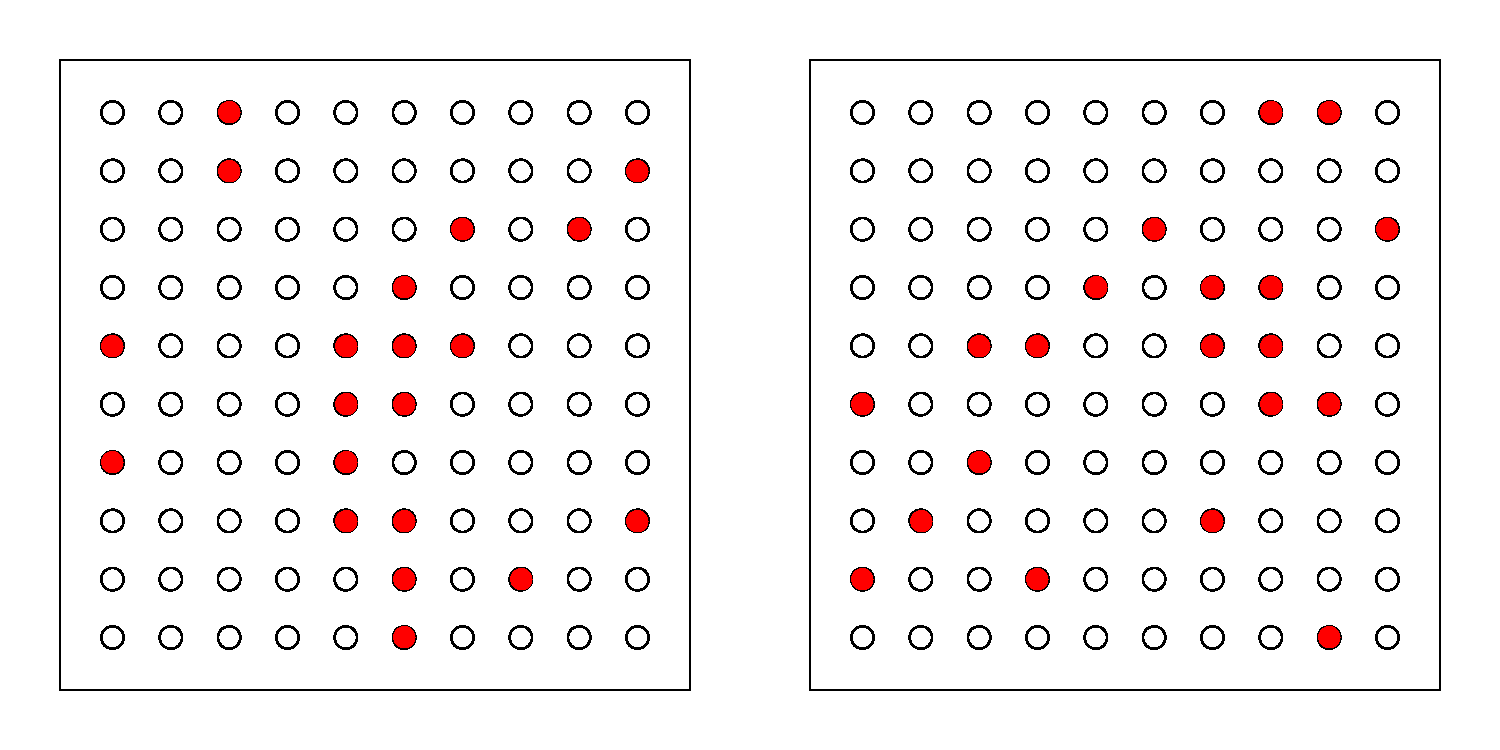
\includegraphics[scale=0.4]{figure/srs.pdf}
\end{figure}
\end{frame}

%---------------------------------------------
\begin{frame}[fragile]{Simple Random Sampling}
Using R to take a SRS of size $n=10$ from a population with $N=100$ cases:
\begin{verbatim}
> sample(1:100, size = 10)
 [1] 48 42 49 77 45 96 33 64 98 65
 
> sample(1:100, size = 10)
 [1] 78 62 58 33 36 15  6 64 41  2
 
> sample(1:100, size = 10)
 [1] 98 40 53 27  8 29  7 84 59 11
\end{verbatim}
%Note by default samples are without replacement.  
\end{frame}

%---------------------------------------------
\begin{frame}{Simple Random Sampling}
\textbf{Example}:  Let \{a,b,c,d,e\} be a population of size $N=5$.  List all possible samples of size $n=2$ from this population.  For SRS what is the probability of selecting each sample of size $n=2$?\\
% \vspace{5cm} 
\vspace{10pt}
\color{blue}
\emph{Solution:}\\
There are 10 possible samples of size $n=2$:\\
$\{a, b\}$; $\{a, c\}$; $\{a, d\}$; $\{a, e\}$; $\{b, c\}$; $\{b, d\}$; $\{b, e\}$;\\ $\{c, d\}$; $\{c, e\}$; $\{d, e\}$\\
\vspace{10pt}
For SRS, $1/10$ is the probability of selecting each sample of size $n=2$.
\end{frame}

%---------------------------------------------
\begin{frame}{Simple Random Sampling}
\color{blue}
Can use combinations to count \# of samples:\\
\vspace{30pt}
$$\binom{5}{2} = \frac{5!}{2!3!} = \frac{5 \cdot 4}{2} = 10$$\\
\vspace{30pt}
In general, there are $\binom{N}{n} = \frac{N!}{n!(N-n)!}$ samples of size $n$ from a population with $N$ cases.
\end{frame}

%---------------------------------------------
\begin{frame}{Simple Random Sampling}
\textbf{Example}:  Suppose a population consists of $N=20$ individuals.  How many possible samples of size $n=4$ can we select from this population?  Assume sampling is done \textbf{without replacement}.\\
% \vspace{5cm}
\vspace{10pt}
\color{blue}
\emph{Solution:}\\
$$\binom{20}{4} = \frac{20!}{4!16!} = \frac{20 \cdot 19 \cdot 18 \cdot 17}{4 \cdot 3 \cdot 2 \cdot 1} = \boxed{4845}$$
\vspace{10pt}

R command:\\
\texttt{> choose(20, 4)}
\end{frame}

%---------------------------------------------
\begin{frame}{Stratified Sampling}
\begin{itemize}
\item For \textbf{stratified sampling} the population is divided into distinct groups called \textbf{strata}.  Then a SRS is selected from from each strata.
\vspace{5pt}
\item The strata are selected so that the cases within each strata are similar in some way.  For example, the strata might be different ethnic or age groups when surveying people.
\vspace{5pt}
\item Commonly used in geographic sampling where the strata can be states or counties.   
\end{itemize}
\end{frame}

%---------------------------------------------
\begin{frame}{Stratified Sampling}
Two stratified random samples.  Cases are grouped into 4 strata, and a SRS of size 4 is selected within each strata. 

\begin{figure}
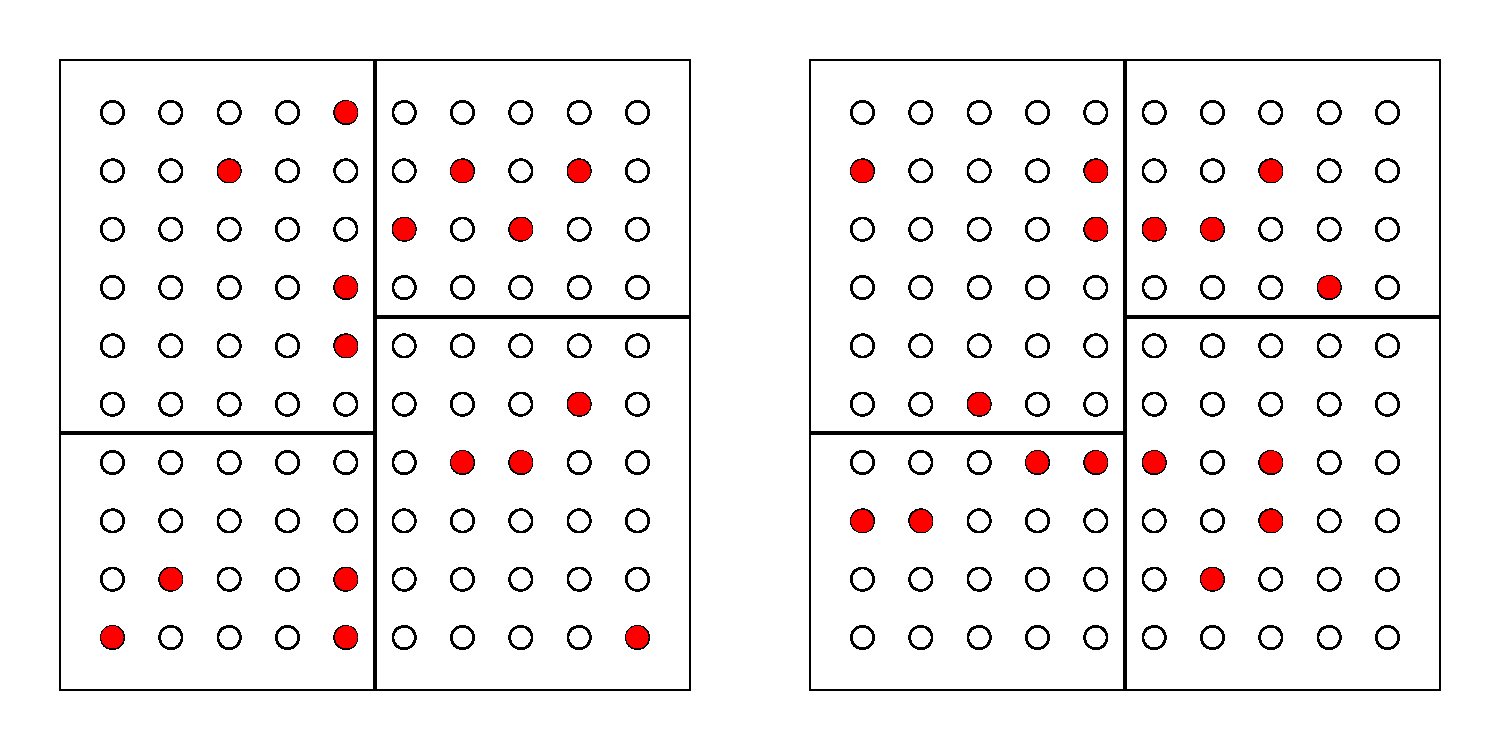
\includegraphics[scale=0.4]{figure/strat.pdf}
\end{figure}
\end{frame}

%---------------------------------------------
\begin{frame}{Cluster Sampling}
\begin{itemize}
\item For \textbf{cluster sampling} the population is divided up into groups called clusters.  Then a fixed number of clusters are randomly sampled, and all cases within each of the selected clusters are included in the sample. 
\vspace{10pt}
\item For example, suppose we want to survey church members.  Instead of taking a SRS of individual church members, we take a random sample of churches (the clusters) and sample all individuals in the selected churches.
\vspace{10pt}
\item Unlike stratified sampling, cluster sampling works best when there is a lot variability within a cluster, and the cases within each cluster are representative of the population.
\end{itemize}
\end{frame}

%---------------------------------------------
\begin{frame}{Cluster Sampling}
Two cluster samples.  There are 25 clusters and 10 clusters are randomly selected.  All cases within each of the selected clusters are included in the sample.  
\begin{figure}
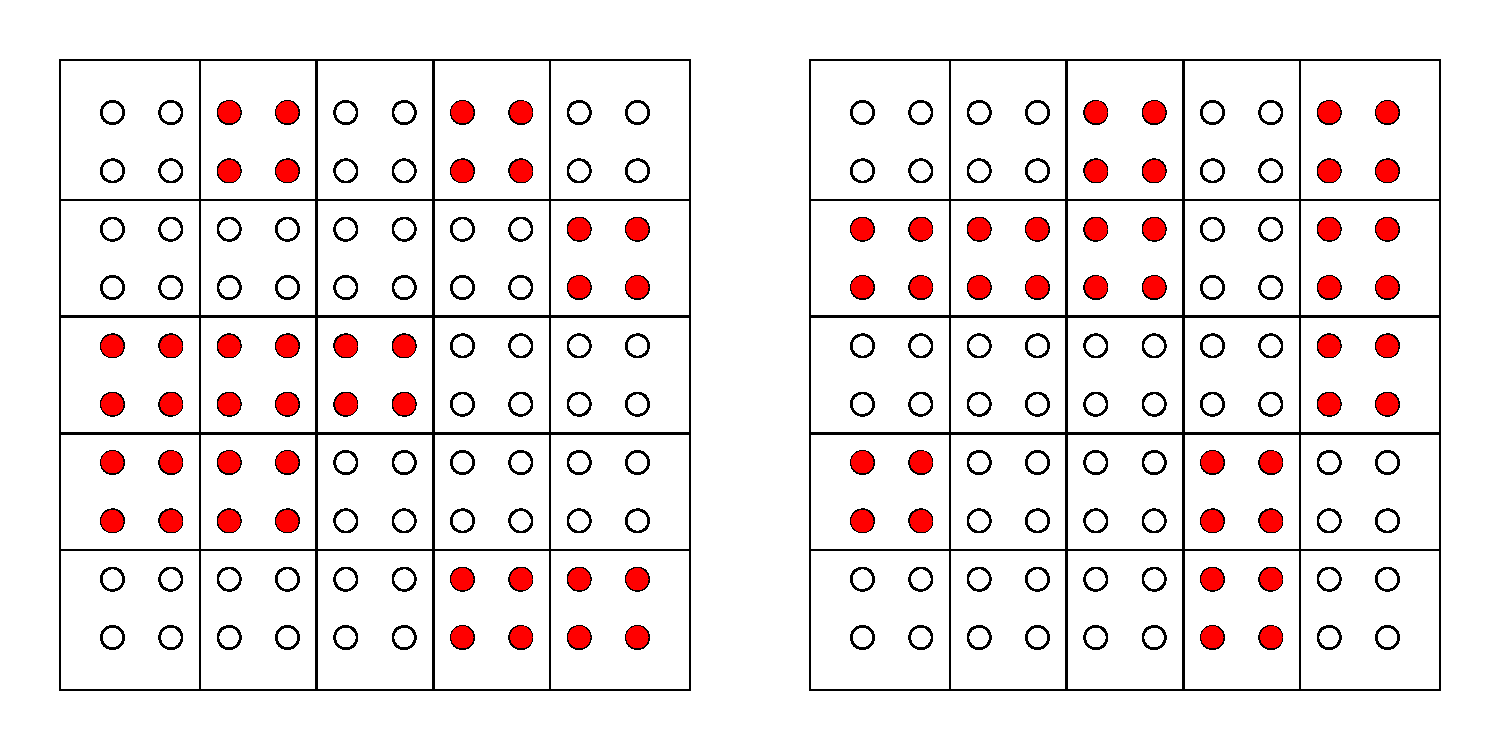
\includegraphics[scale=0.4]{figure/clust.pdf}
\end{figure}
\end{frame}

%---------------------------------------------
\begin{frame}{Systematic Sampling}
\begin{itemize}
\item A \textbf{systematic sample} is drawn by selecting cases systematically from a sample frame.
\vspace{10pt}
\item For example, suppose we have a alphabetical list of names of all students attending CSUEB.  We then select a student at the beginning of the list and proceed to select every 10th name thereafter.  
\end{itemize}
\end{frame}

%---------------------------------------------
\begin{frame}{Systematic Sampling}
A systematic sample.  Every third case is included in the sample.  
\begin{figure}
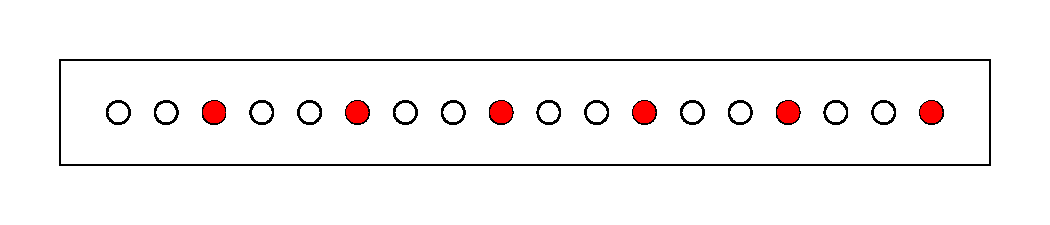
\includegraphics[scale=0.6]{figure/sys.pdf}
\end{figure}
\end{frame}

\begin{frame}{Census}
\begin{itemize}
\item A \textbf{census} is taken if every individual in the population is included in the sample.  That is, the sample and the population are the same.
\vspace{5pt}
\item Taking a census is more costly and time consuming than random sampling.
\vspace{5pt}
\item For large populations, data collection and processing for a census is complex and may be prone to errors.
\end{itemize}
\end{frame}

%---------------------------------------------
\begin{frame}{Example}
Identify the type of sampling design:\\
\vspace{10pt}
\begin{itemize}
\item The selection of 200 people to serve as potential jurors in a trail is conducted by assigning a number to each of 140,000 registered voters in the county.  The R command \texttt{sample(1:140000, 200)} is used to take a sample of 200 numbers between 1 and 140,000.  People having these 200 numbers are sent postcards notifying them of jury duty.\\
{\color{blue} \emph{Ans:} Simple random sampling (SRS)}
\vspace{5pt}
\item Suppose you are selecting microchips from a production line for inspection.  As the chips process past the inspection point, every 100th chip is selected for inspection.\\
{\color{blue} \emph{Ans:} Systematic sampling}
\end{itemize} 
\end{frame}

%---------------------------------------------
\begin{frame}{Example}
Identify the type of sampling design:\\
\vspace{10pt}
\begin{itemize}
\item In a survey on household income, 1000 households are randomly selected in each of the 50 states in the U.S.\\
{\color{blue} \emph{Ans:} Stratified sampling}
\vspace{5pt}  
\item A survey is conducted to find the average weight of cows in a region.  A list of all farms is available for the region, and 50 farms are selected at random.  Then the weight of each cow at the 50 selected farms is recorded.\\
{\color{blue} \emph{Ans:} Cluster sampling}
\end{itemize}
\end{frame}

%---------------------------------------------
\begin{frame}{Problems with Survey Sampling}
A sample is \textbf{biased} if it is not representative of the population.  Statistics from biased samples tend to overestimate or underestimate the population parameter.  Some sources of bias for survey sampling include:\\
\begin{itemize}
\item \textbf{Nonresponse}: failing to obtain responses from some individuals selected for the sample.  There may be differences between those that respond and do not respond to a survey.  
\item Taking a \textbf{sample of convenience} by only including individuals that are easily accessible in the sample.
\item Allowing the sample to consist entirely of volunteers.
\item Wording a survey question in such a way that it influences the response.
\item \textbf{Undercoverage}: Using a sample frame that does not include a portion of the population.
\end{itemize}
\end{frame}

%---------------------------------------------
\begin{frame}{Historical Example: Landon vs. FDR, 1936}
\begin{itemize}
\item Literary Digest polled 10 million Americans, and 2.4 million responded
\item Prediction: 43\% for FDR
\item Result: 62\% for FDR
\begin{figure}
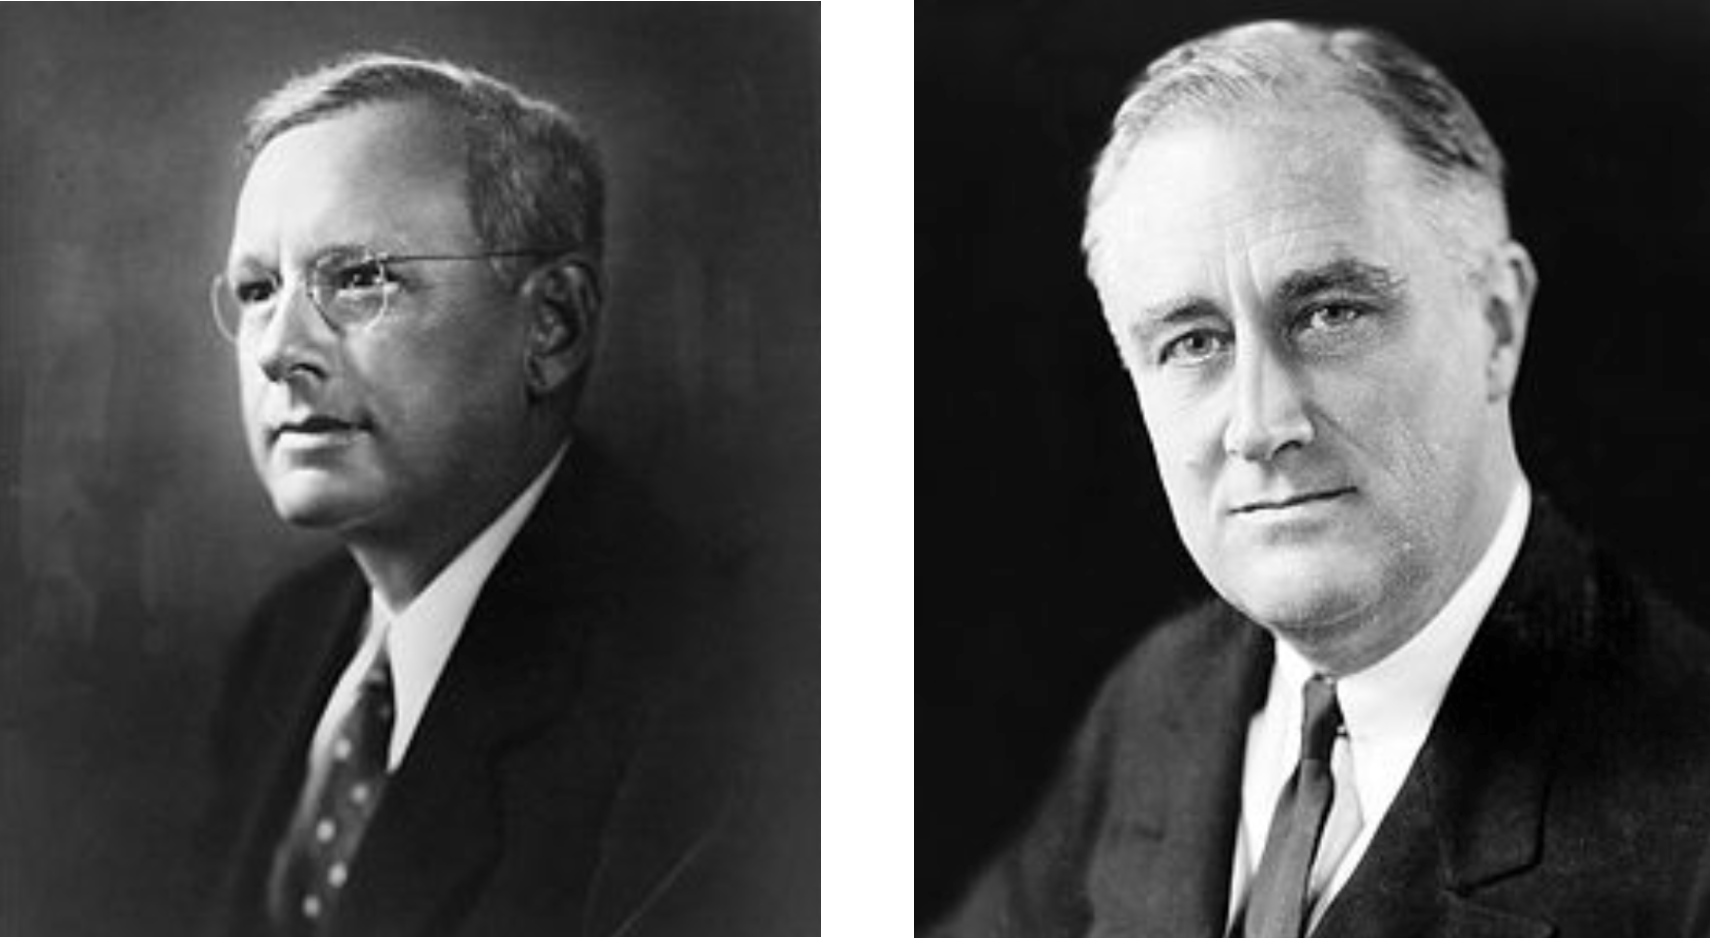
\includegraphics[scale=0.2]{figure/landon-fdr.png}
\end{figure}
\item The magazine was so discredited by the poll that is was discontinued.
\end{itemize}
\end{frame}

%---------------------------------------------
\begin{frame}{Historical Example: Landon vs. FDR, 1936}
What went wrong?
\vspace{10pt}
\begin{itemize}
\item The magazine had surveyed
\begin{itemize}
\item its own readers,
\item registered automobile owners, and
\item registered telephone users.
\end{itemize}
\vspace{5pt}
\item The sample frame consisted of individuals that were wealthier than the majority of voters, and therefore more likely to support the Republicans (example of undercoverage).  
\vspace{5pt}
\item Nonresponse: 10 million sampled, but 2.4 million responded.  Persons supporting Landon were more likely to have responded to the survey.    
\end{itemize}
\end{frame}




\end{document}